\documentclass[letterpaper, twoside, 12pt]{book}

\usepackage{amsmath,amsfonts, amsthm}
\usepackage{yfonts}
\usepackage{amsrefs}
\usepackage{fancyhdr}
\usepackage{graphicx}
\usepackage{float}
\usepackage[margin=1in]{geometry}
\usepackage{array}
\usepackage{esint}
\usepackage{harpoon}
\usepackage{stmaryrd}
\usepackage{multicol}
\usepackage{multirow}
\usepackage{pgf,tikz}
\usetikzlibrary{arrows}

\usepackage{makeidx}
\makeindex

\definecolor{AuburnOrange}{RGB}{221,85,12}
\definecolor{AuburnBlue}{RGB}{3,36,77}
\definecolor{AuburnSecondaryBlue}{RGB}{73,110,156}
\definecolor{AuburnSecondaryOrange}{RGB}{246,128,38}
\definecolor{AlabamaCrimson}{RGB}{163,38,65}
\definecolor{LSUpurple}{RGB}{70,29,124}
\definecolor{VanderbiltGold}{RGB}{207,181,59}

\usepackage[pdfpagelabels]{hyperref}
\hypersetup{colorlinks=true,linkcolor=AuburnSecondaryOrange}

% \usepackage[tracking]{microtype}
% \UseMicrotypeSet{all}
% \SetTracking[spacing = {35*,0*,0*}]{encoding = *}{7}
% \linespread{1.025}

\def\scaleint#1{\vcenter{\hbox{\scaleto[3ex]{\displaystyle\int}{#1}}}}
\def\bs{\!\!}

\renewcommand{\arraystretch}{1.5}

\pagestyle{fancy} \headheight 14.49998pt

\newcommand{\tstamp}{\today}
\renewcommand{\chaptermark}[1]{\markboth{#1}{}}
\renewcommand{\chaptermark}[1]{\markright{#1}}

\lhead[\fancyplain{}{Clontz \thepage}]         {\fancyplain{}{\scshape\nouppercase{\rightmark}}}

\chead[\fancyplain{}{}]
{\fancyplain{}{}}


\rhead[\fancyplain{}{Calculus II Lecture Notes}]       {\fancyplain{}{Clontz \thepage}}

\lfoot[\fancyplain{}{Auburn University}]                 {\fancyplain{\tstamp}{\tstamp}}

\cfoot[\fancyplain{\thepage}{}]         {\fancyplain{\thepage}{}}

\rfoot[\fancyplain{\tstamp} {\tstamp}]  {\fancyplain{}{Auburn University}}

\theoremstyle{definition}
\newtheorem{theorem}{Theorem}

% \theoremstyle{plain}
\newtheorem{proposition}[theorem]{Proposition}
\newtheorem{recall}[theorem]{Recall}

\theoremstyle{definition}
\newtheorem{definition}[theorem]{Definition}
\newtheorem{notation}[theorem]{Notation}
\newtheorem{goal}[theorem]{Goal}
\newtheorem{motivation}[theorem]{Motivation}
\newtheorem{remark}[theorem]{Remark}
\newtheorem{TrueFact}[theorem]{True Fact}
\newtheorem{FalseFact}[theorem]{False Fact}
\newtheorem{conjecture}[theorem]{Conjecture}
\newtheorem{conclusion}[theorem]{Conclusion}
\newtheorem{observation}[theorem]{Observation}
\newtheorem{problem}[theorem]{Problem}
\newtheorem{question}[theorem]{Question}
\newtheorem{example}[theorem]{Example}
\newtheorem{note}[theorem]{Note}
\newtheorem{convention}[theorem]{Convention}
\newtheorem{eqn}[theorem]{Equation}
\newtheorem{strategy}[theorem]{Strategy}
\newtheorem{properties}[theorem]{Properties}
\newtheorem{corollary}[theorem]{Corollary}

\newcommand{\HRule}{\rule{\linewidth}{0.5mm}}
\newcommand{\harpvec}[1]{\overrightharp{\ensuremath{\mathbf{#1}}}}
\newcommand*{\threevec}[3]{\ensuremath{\left\langle #1, #2, #3 \right\rangle}}
\newcommand*{\twovec}[2]{\ensuremath{\left\langle #1, #2 \right\rangle}}
\newcommand*{\unitvec}[1]{\ensuremath{\mathbf{\widehat{#1}}}}
\newcommand{\veci}{\ensuremath{\mathbf{\widehat{i}}}}
\newcommand{\vecj}{\ensuremath{\mathbf{\widehat{j}}}}
\newcommand{\veck}{\ensuremath{\mathbf{\widehat{k}}}}
\newcommand{\ds}{\ensuremath{\displaystyle}}


\newcommand{\contrasymb}{\mathrel{\raisebox{.1em}{\reflectbox{\rotatebox[origin=c]{220}{$\lightning$}}}}}

\newenvironment{answer}{\paragraph{Answer.}}{\hfill$\blacklozenge$}
\newenvironment{contraproof}{\paragraph{Proof.}}{\hfill$\contrasymb$}

\begin{document}

\setcounter{chapter}{5}

\chapter{Applications of Integrals}

\section{Area Between Curves}

\subsection{Area with Respect to the \emph{x}-axis}

\begin{figure}[H]
\centering
%tikz Picture
\definecolor{ffzztt}{rgb}{0.6,0.6,0.6}
\definecolor{wwqqqq}{rgb}{0.13,0.13,0.13}
\definecolor{qqqqcc}{rgb}{0.27,0.27,0.27}
\definecolor{qqzzqq}{rgb}{0.2,0.2,0.2}
\begin{tikzpicture}[line cap=round,line join=round,>=triangle 45,x=1.0cm,y=1.0cm]
\draw[->,color=black] (-2.97,0) -- (3.18,0);
\foreach \x in {-2,-1,1,2,3}
\draw[shift={(\x,0)},color=black] (0pt,2pt) -- (0pt,-2pt) node[below] {\footnotesize $\x$};
\draw[->,color=black] (0,-0.46) -- (0,7.12);
\foreach \y in {1,2,3,4,5,6,7}
\draw[shift={(0,\y)},color=black] (2pt,0pt) -- (-2pt,0pt) node[left] {\footnotesize $\y$};
\draw[color=black] (0pt,-10pt) node[right] {\footnotesize $0$};
\clip(-2.97,-0.46) rectangle (3.18,7.12);
\draw[line width=1.5pt,color=black] (-1.73,4.07) -- (-1.73,1.93) -- (-1.04,1.93) -- (-1.04,4.07) -- cycle;
\fill[line width=2.4pt,color=ffzztt,fill=ffzztt,fill opacity=0.3] (-1.73,4.07) -- (-1.73,1.93) -- (-1.04,1.93) -- (-1.04,4.07) -- cycle;
\draw[line width=1.5pt,color=black] (-1.04,5.52) -- (-1.04,0.48) -- (-0.35,0.48) -- (-0.35,5.52) -- cycle;
\fill[line width=2.4pt,color=ffzztt,fill=ffzztt,fill opacity=0.3] (-1.04,5.52) -- (-1.04,0.48) -- (-0.35,0.48) -- (-0.35,5.52) -- cycle;
\draw[line width=1.5pt,color=black] (-0.35,6) -- (-0.35,0) -- (0.35,0) -- (0.35,6) -- cycle;
\fill[line width=2.4pt,color=ffzztt,fill=ffzztt,fill opacity=0.3] (-0.35,6) -- (-0.35,0) -- (0.35,0) -- (0.35,6) -- cycle;
\draw[line width=1.5pt,color=black] (0.35,5.52) -- (0.35,0.48) -- (1.04,0.48) -- (1.04,5.52) -- cycle;
\fill[line width=2.4pt,color=ffzztt,fill=ffzztt,fill opacity=0.3] (0.35,5.52) -- (0.35,0.48) -- (1.04,0.48) -- (1.04,5.52) -- cycle;
\draw[line width=1.5pt,color=black] (1.04,4.09) -- (1.04,1.91) -- (1.73,1.91) -- (1.73,4.09) -- cycle;
\fill[line width=2.4pt,color=ffzztt,fill=ffzztt,fill opacity=0.3] (1.04,4.09) -- (1.04,1.91) -- (1.73,1.91) -- (1.73,4.09) -- cycle;
\draw[line width=2pt,color=qqzzqq, smooth,samples=100,domain=-2.9700384090603635:3.176476820910142] plot(\x,{(\x)^2});
\draw[line width=2pt,color=qqqqcc, smooth,samples=100,domain=-2.9700384090603635:3.176476820910142] plot(\x,{6-(\x)^2});
\draw (-2.55,7.12) node[anchor=north west] {$ApproximateArea \, = \,14.13$};
\draw (-1.92,6.68) node[anchor=north west] {$ExactArea \, = \,13.86$};
\begin{scriptsize}
\draw[color=wwqqqq] (-1.65,-0.26) node {Start};
\draw[color=wwqqqq] (1.92,-0.22) node {End};
\end{scriptsize}
\end{tikzpicture}
% End Tikz Picture
\caption{Area Between Two Curves}
\label{AreaBetweenCurvesPic}
\end{figure}

\begin{goal}
 To be able to find the area between two curves.
\end{goal}

\begin{motivation}
Say we want to find the area enclosed by two curves.  Over a given area, there is a top function and a bottom function.  Let's call the top function $f(x)$ and the bottom function $g(x)$.  Just as we did with area under the curve, we can split this region into $n$ rectangles and add up all of their areas to approximate the area between these curves.  Each rectangle has width $\Delta x$.  To find the length of each rectangle, let $x_i^*$ denote a point within the $i^{\rm th}$ rectangle.  Then the length (or height) of rectangle $i$ is $f(x_i^*) - g(x_i^*)$.
\end{motivation}

\begin{theorem}
The area, $A$, between two curves can be found by
$$A = \lim_{n \rightarrow \infty} \sum_{i = 1}^{n} \left( f\left(x_i^*\right) - g\left(x_i^*\right) \right) \, \Delta x.$$
\end{theorem}

\begin{recall}
 From Chapter $5.3$, we have seen that $$A = \lim_{n \rightarrow \infty} \sum_{i=1}^{n} f\left(x_i^*\right) \, \Delta x = \int_a^b f(x) \, dx.$$
\end{recall}

Following the same line of reasoning, we have

\begin{theorem}\index{Area Between Curves}
The area $A$ of the region bounded by the curves $y = f(x), y = g(x), x = a$ and $x = b,$ where $f$ and $g$ are continous functions such that $f(x) \geq g(x)$ for all $x \in \left[a,b\right]$ is $$A = \lim_{n \rightarrow \infty} \sum_{i = 1}^{n} \left( f\left(x_i^*\right) - g\left(x_i^*\right) \right) \, \Delta x = \int_a^b f(x) - g(x) \, dx.$$
\emph{(Think: ``Top minus Bottom'')}
\end{theorem}

\begin{problem}
 Find the area of the region bounded above by $y = e^x$, below by $y = x$, and on the sides by $x = 0$ and $x = 1$.
\end{problem}

\newpage

\begin{problem}
 Find the area bounded by $y = x^2$ and $y = 2x-x^2$.
\end{problem}

\vfill

\begin{problem}
 Find the area bounded by $y = \sin(x)$ and $y = \cos(x)$ from $x = 0$ to $x = \frac{\pi}{2}$.
\end{problem}

\vfill

\newpage

\subsection{Area with Respect to the \emph{y}-axis}

Finding the area with respect to the $y$-axis is very similar.  One simply has to tilt his or her head to the right.  That is to say that instead of thinking ``Top Minus Bottom,'' think ``Right minus Left.''

\begin{problem}
 Find the area enclosed by $y = x-1$ and $y^2 = 2x+6$.
\end{problem}

\vfill

\begin{problem}
 Find the area enclosed by $x = 2y-y^2$ and $x = y^2-4y$.
\end{problem}

\vfill

\noindent Suggested Homework: Section $6.1$ numbers $1,$ $4,$ $12,$ $24,$ $27,$ $44,$ $50$

% \newpage

% \section{Volume Using the Disc/Washer Method}

% \begin{motivation}
%  Just as we used rectangles to approximate area under a curve in $\mathbb{R}^2$, we will use \emph{right circular cylinders} to approximate the volume of a solid in $\mathbb{R}^3$.
% \end{motivation}

% \begin{recall}\index{Volume of Cylinder}
%  The volume of a right circular cylinder is the area of the base $A$ times the height of the cylinder $h$.  That is to say $$V_{\mbox{cylinder}} = Ah.$$
% \end{recall}

% \begin{strategy}
%  So, we will be
%  \begin{itemize}
%   \item Cutting a solid $S$ into cylindrical cross sections,
%   \item Finding the volume of each cross section, and
%   \item adding them all up.
%  \end{itemize}
% That is to say that $$V(S) \approx \sum_{i=1}^n A(x_i^*)\Delta x.$$
% \end{strategy}

% \begin{observation}
%  It should be noted that the more cylindrical cross sections, the closer the approximation will be.
% \end{observation}


% \begin{definition}[Disc Method\index{Disc Method}]
%  Let $S$ be a solid that lies between $x=a$ and $x=b$.  If the cross sectional area of $S$ in the plane $P_x$ through $x$ and perpendicular to the $x$-axis is $A(x)$, where $A$ is a continuous function, then the \textbf{volume} of $S$ is $$V(S) = \lim_{n \rightarrow \infty} \sum_{i=1}^n A\left(x_i^*\right) \Delta x = \int_a^b A(x) \, dx.$$
% \end{definition}


% \begin{figure}[H]
%  \centering
%  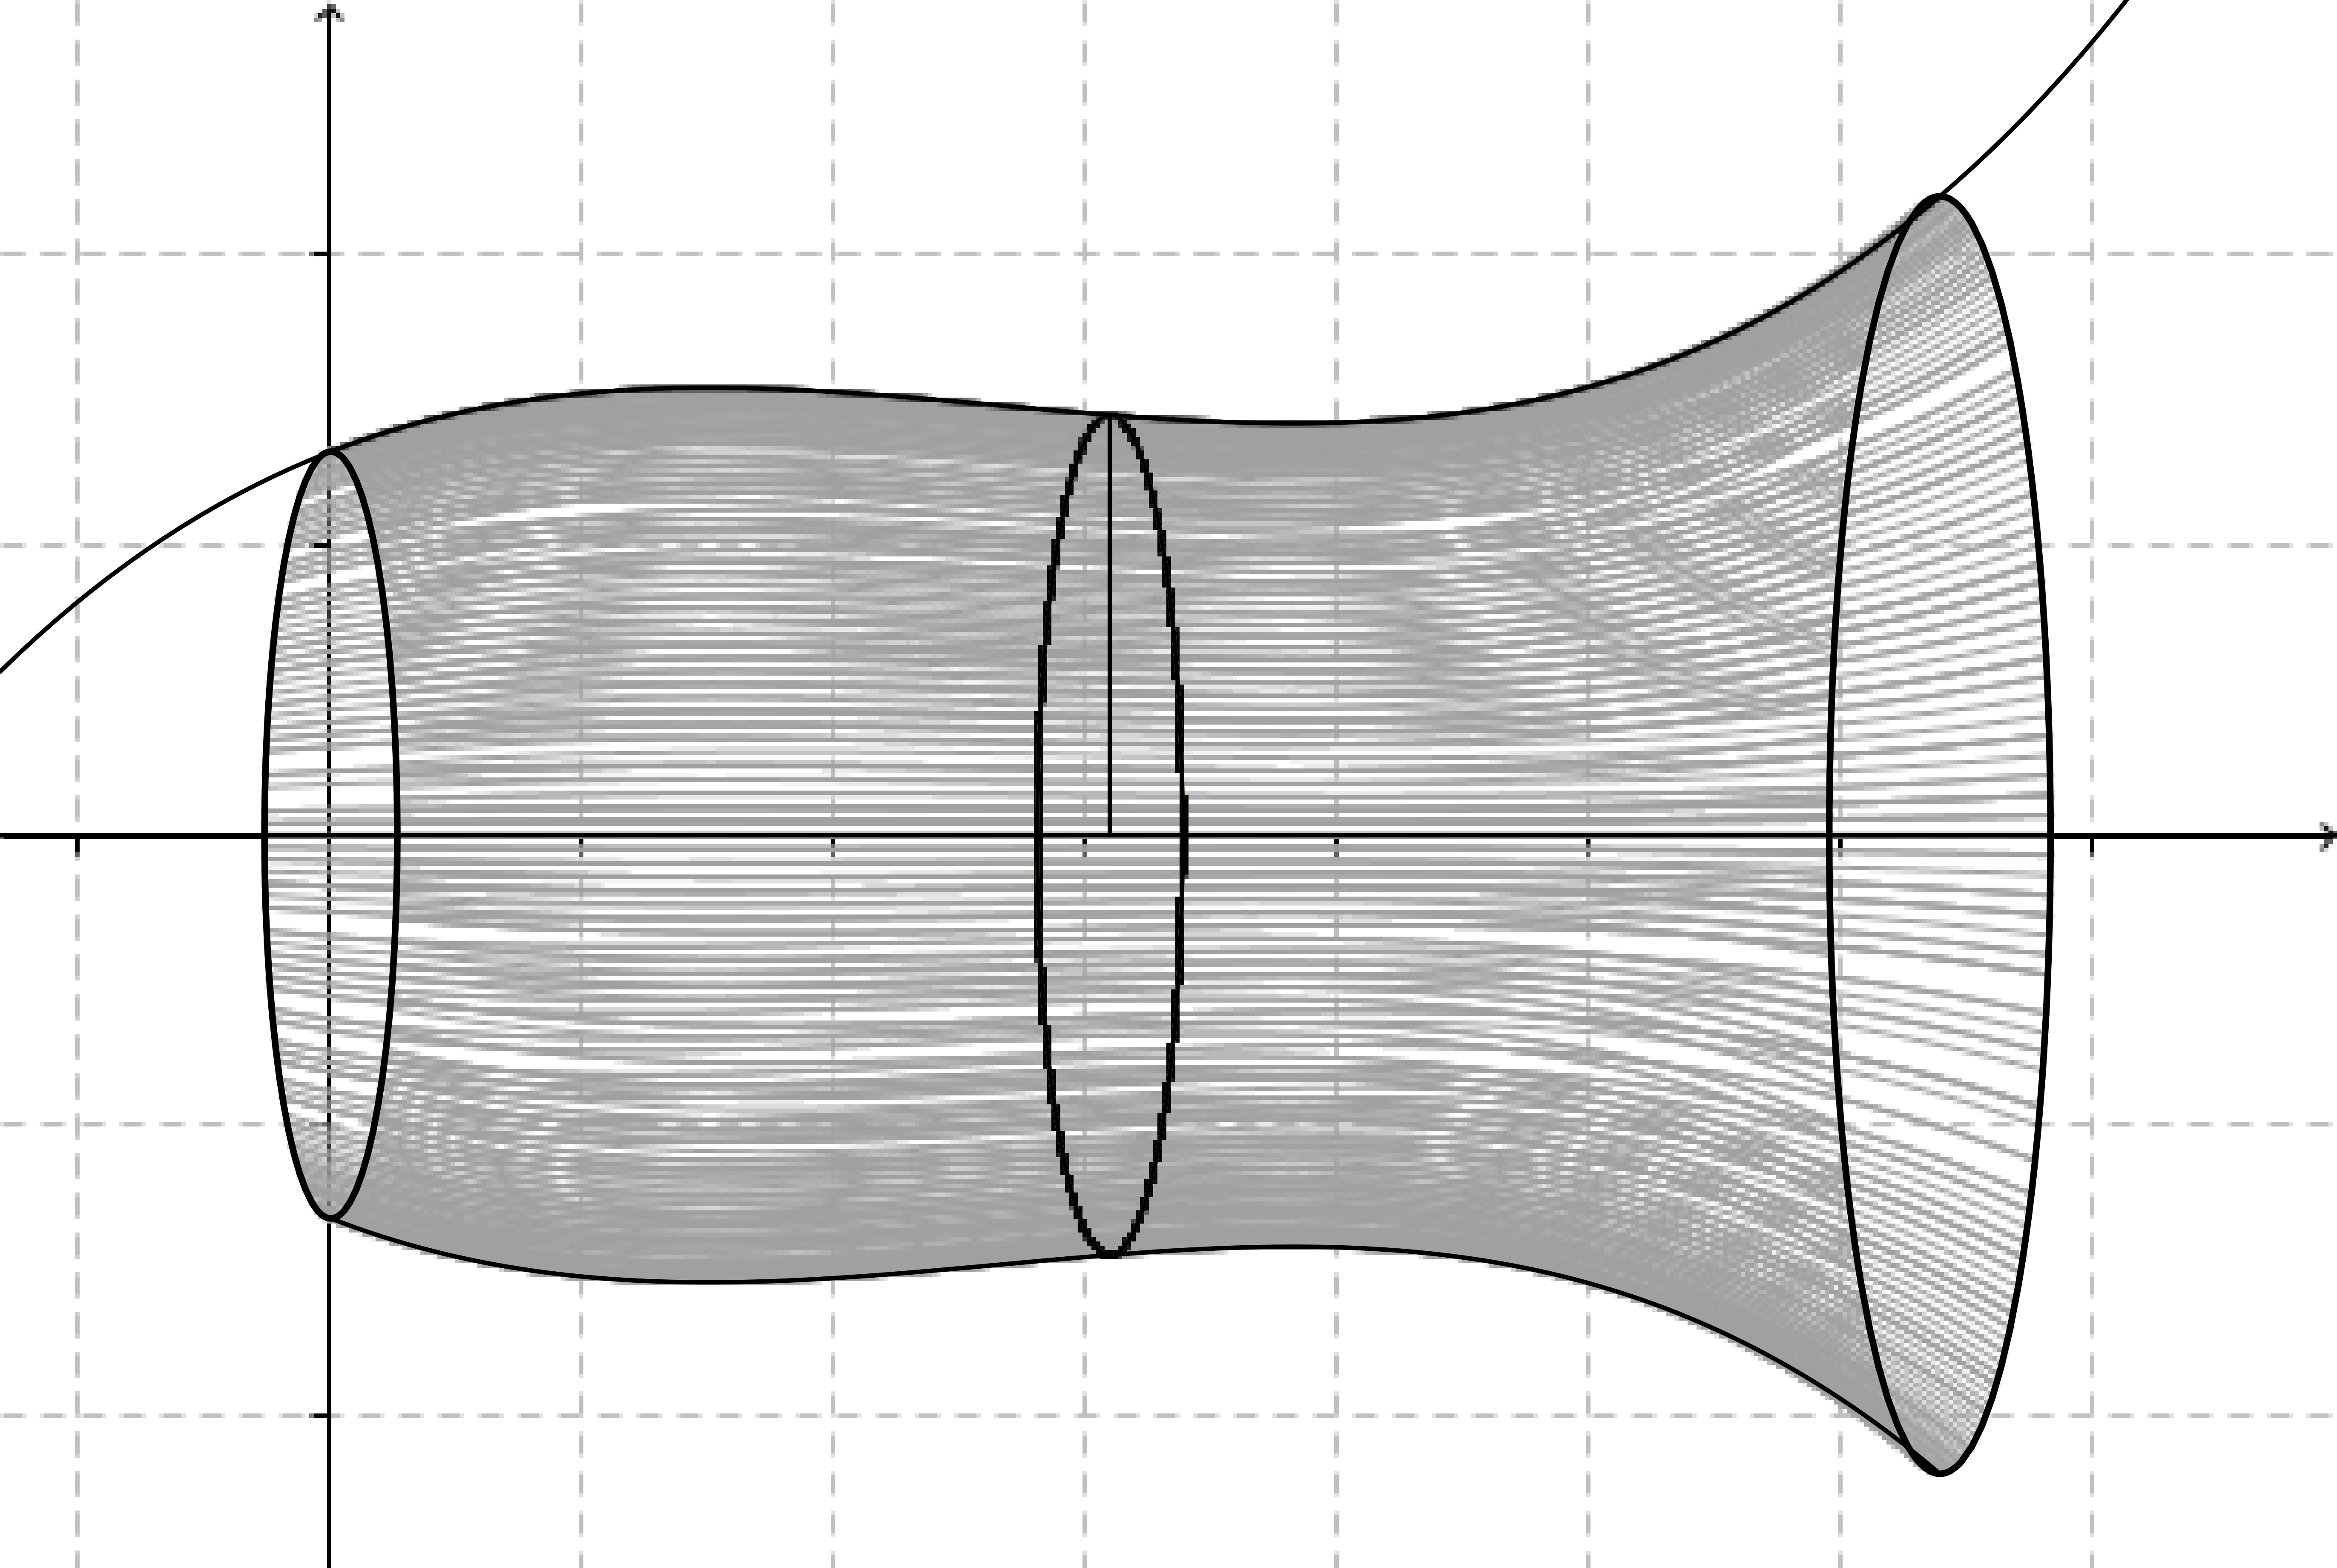
\includegraphics[width=3in]{DiscMethodLectureNotes.png}
%  \caption{Disc Method}
%  \label{DiscMethodFigure}
% \end{figure}

% \newpage

% \begin{problem}
%  Show that the volume of a sphere of radius $r$ is $\ds V = \frac{4}{3}\pi r^3$.
% \end{problem}

% \vfill

% \begin{problem}
%  Find the volume of the solid obtained by rotating the curve $y=\sqrt{x}$ about the $x$-axis from $x = 0$ to $x = 1$.
% \end{problem}

% \vfill

% \newpage

% \begin{problem}[Gabriel's Horn Pt. I\index{Gabriel's Horn Volume}]
%  Find the volume of the solid obtained by rotating the curve $\ds y=\frac{1}{x}$ about the $x$-axis from $1$ to an arbitrary point $a > 1.$  What happens as $a$ gets extremely large?
% \end{problem}

% \vfill

% \begin{problem}
%  Find the volume of the solid obtained by rotating the curve $y = x^3$ bounded by $y = 0$ and $y=8$ about the $y$-axis.
% \end{problem}

% \vfill

% \newpage

% \begin{figure}[H]
%  \centering
%  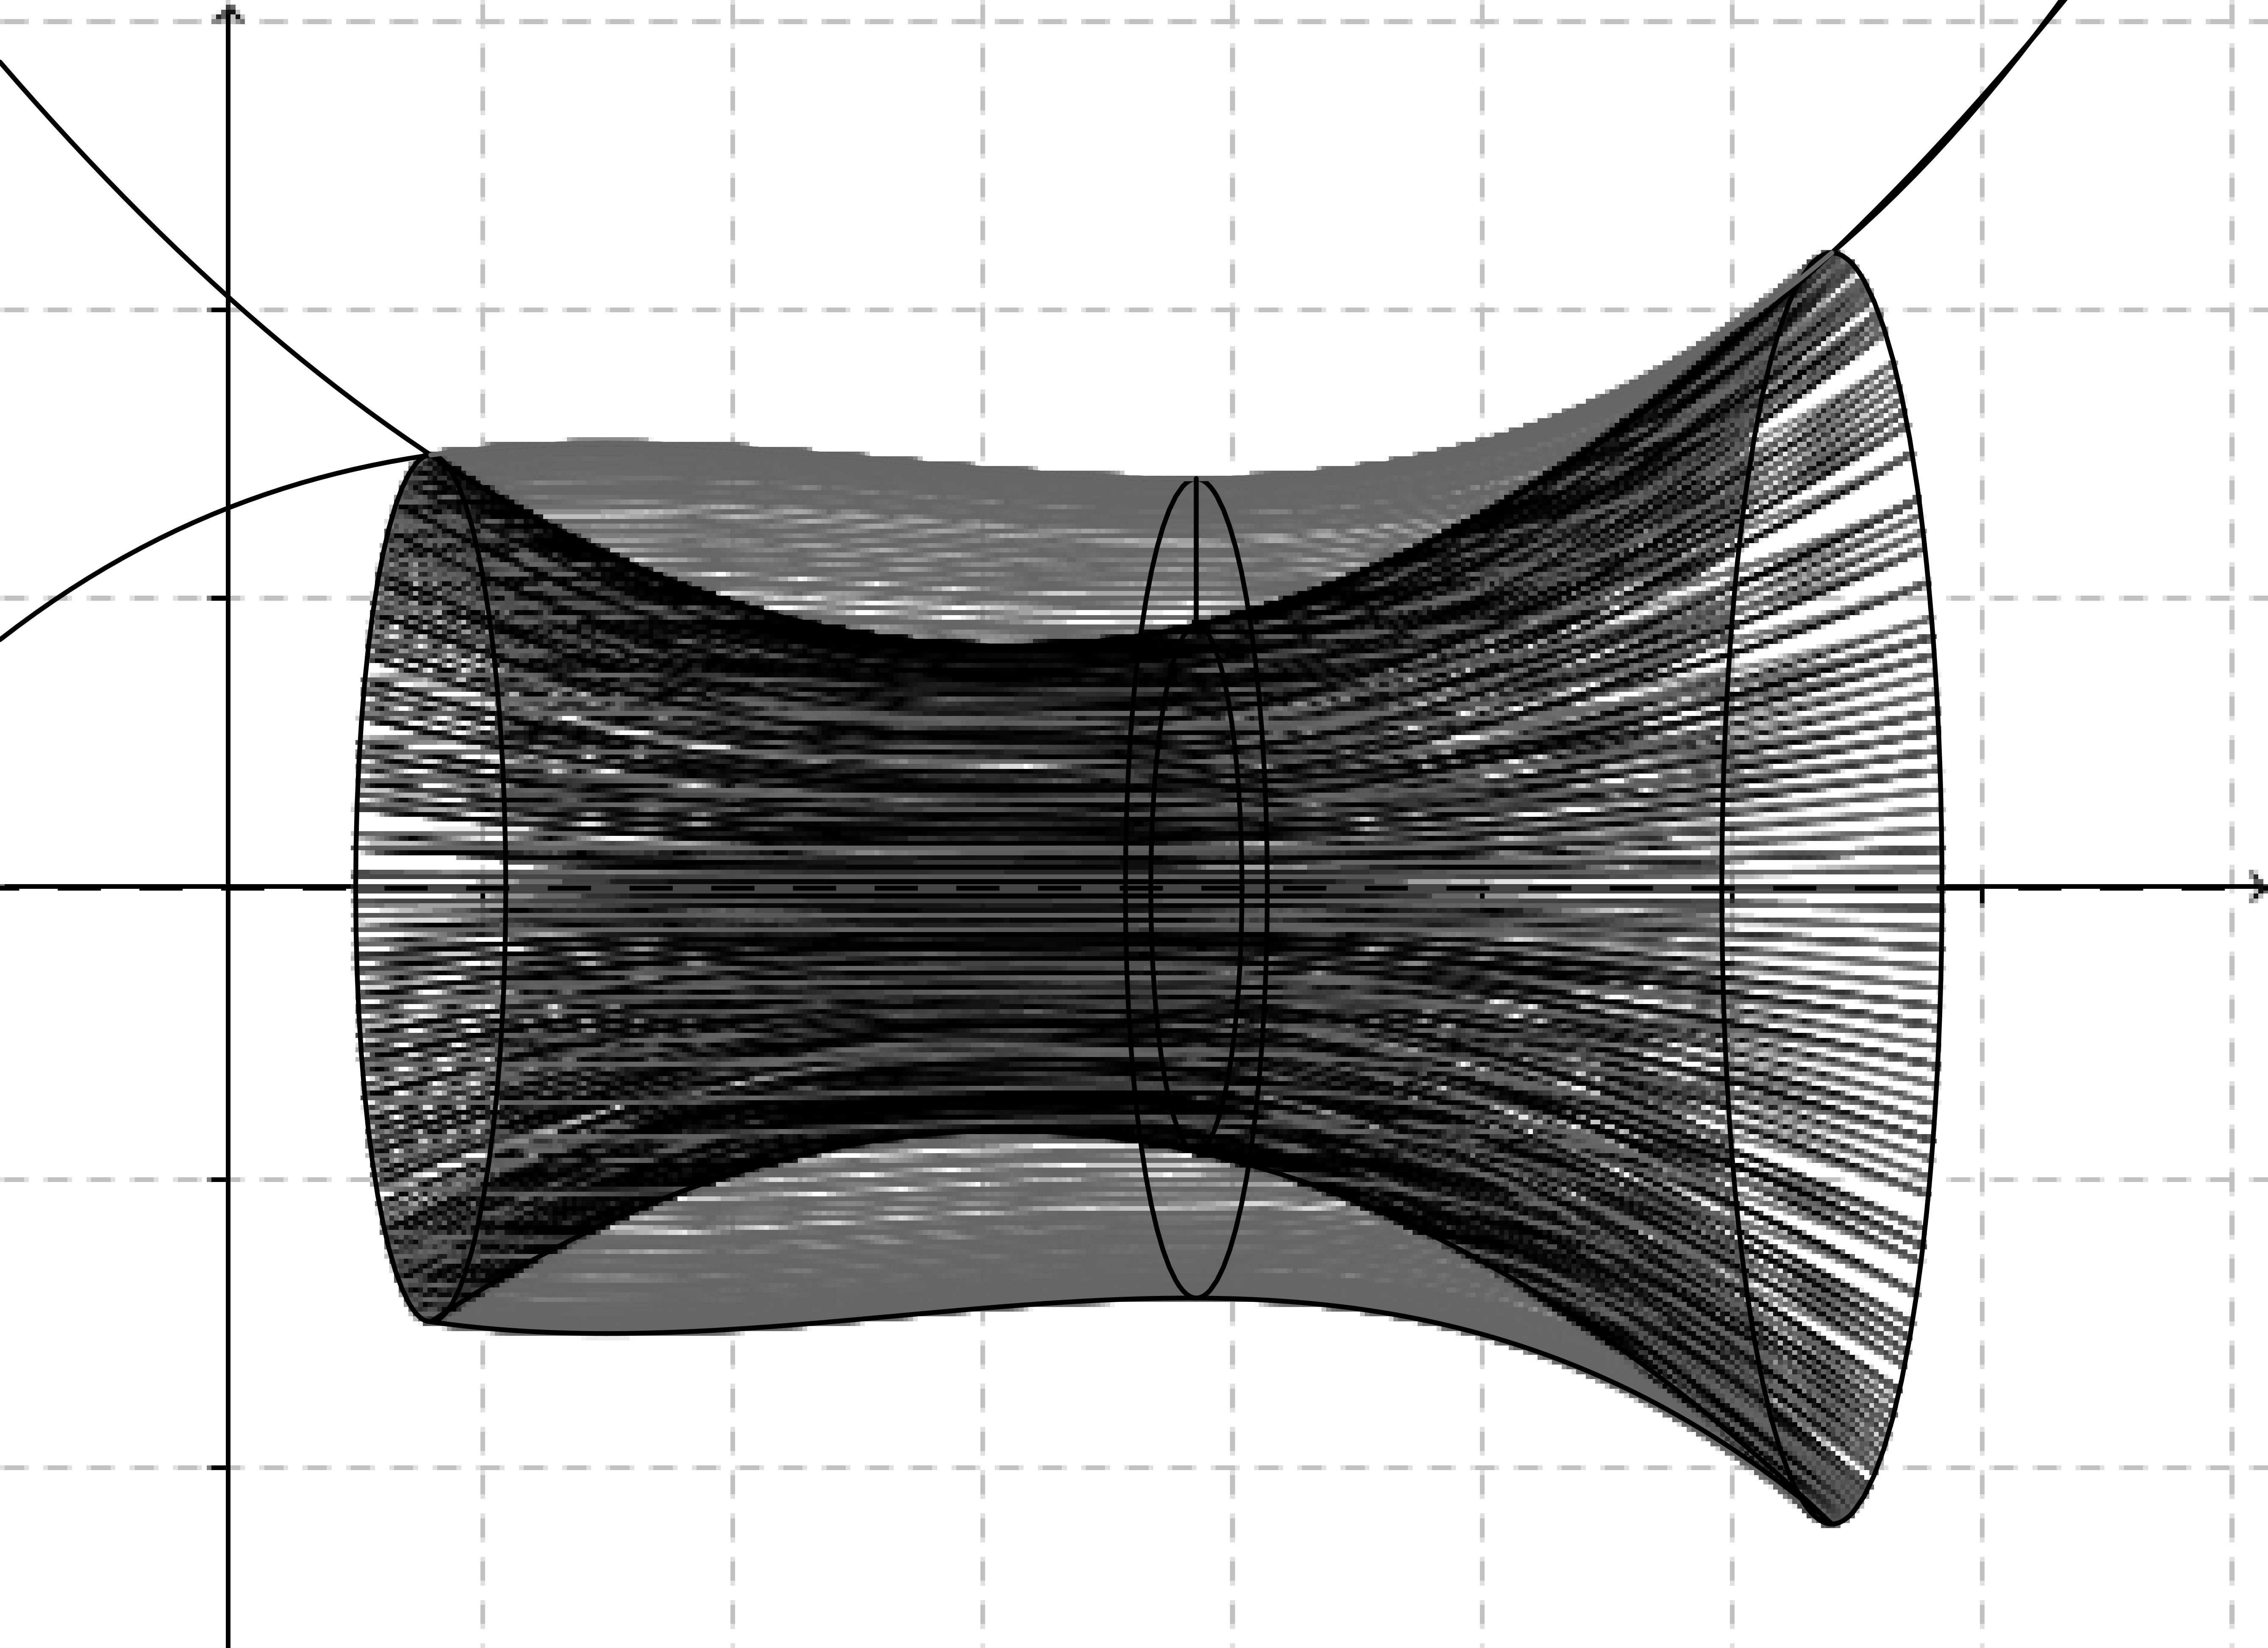
\includegraphics[width=3in]{WasherMethodLectureNotes.png}
%  \caption{Washer Method}
%  \label{WasherMethodFigure}
% \end{figure}

% \begin{motivation}
%  What if we wanted to rotate the area between two functions around the $x$-axis or $y$-axis?  That shape would look like a washer as depicted in Figure \ref{WasherMethodFigure}.
% \end{motivation}

% \begin{problem}\index{Washer Method}
%  Given the outer radius of the disc is length $R$ from the axis of rotation and the inner circle of the disc is of length $r$ from the axis of rotation, what is the area of the base of the disc?
% \end{problem}

% \vfill

% \begin{problem}
%  Find the volume of the surface produced by rotating the region bounded by $y=x$ and $y=x^2$ about the line $x = -1$.
% \end{problem}

% \vfill

% \noindent Suggested Homework: Section $6.2$ numbers $4,$ $5,$ $12,$ $15,$ $19,$ $25,$ $42,$ $54,$ $56,$ $59$
% \newpage

% \section{Volume by Cylindrical Shell}

% \begin{figure}[H]
%  \centering
%  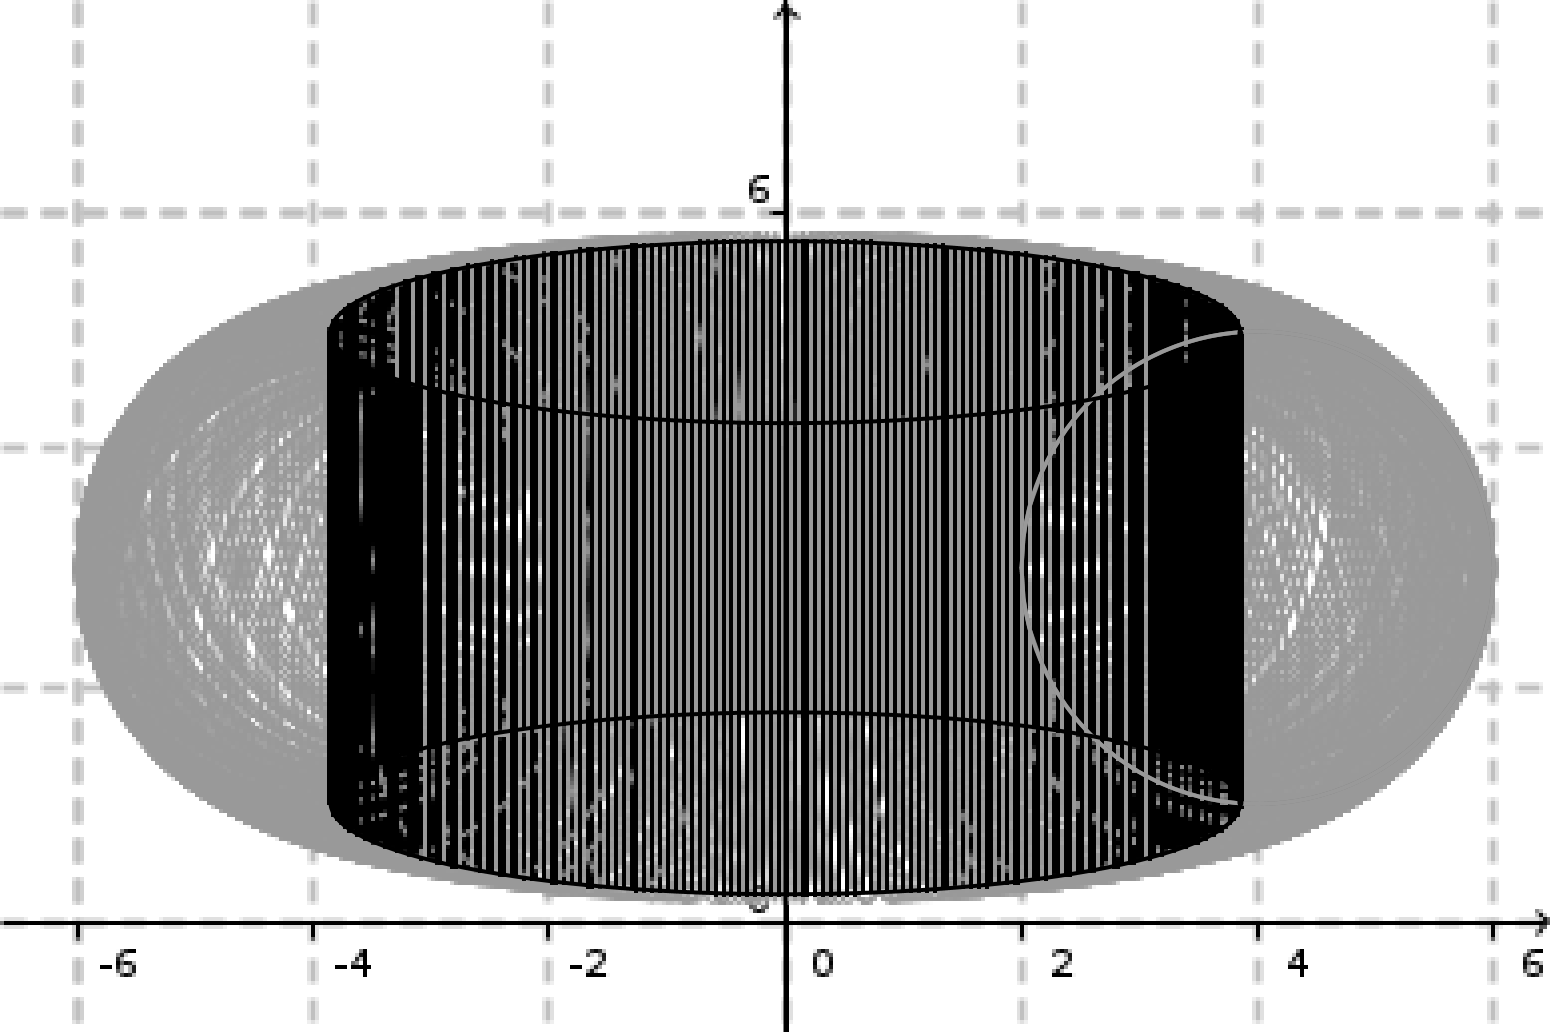
\includegraphics[width=3in]{ShellMethodLectureNotes.png}
%  \caption{Shell Method}
%  \label{ShellMethodFigure}
% \end{figure}

% \begin{motivation}
%  Sometimes it is easier to deal with cylindrical shells rather than discs.  When this happens, what we want to do is peal away sections of this surface one layer at a time, much like layers of an onion (not to be confused with \emph{The Onion}).  In this case, each layer can be straightened out and placed on a table so that it looks like a rectangular prism, which has volume length times width times height.  The length of the shell is the circumference of the shell, the length is the height, and the width is $\Delta x$.  This width will become arbitrarily small with the integration.
% \end{motivation}

% \begin{theorem}[Shell Method\index{Shell Method}]
%  The volume of a solid rotated about the $y$-axis under the curve $y = f(x)$ from $y = a$ to $y = b$ is $V = \int_a^b 2\pi x f(x) \, dx$.
% \end{theorem}

% \begin{problem}
%  Find the volume of the solid obtained by rotating $y = 2x^2-x^3$ and $y = 0$ about the $y$-axis.
% \end{problem}

% \vfill

% \begin{problem}
%  Find the volume of the solid obtained by rotating $y = x$ and $y = x^2$ about the $y$-axis.
% \end{problem}

% \vfill

% \newpage

% \begin{problem}
%  Find the volume of the solid obtained by rotating $y = \sqrt{x}$  about the $x$-axis from $y = 0$ to $y = 1$.
% \end{problem}

% \vfill

% \begin{problem}
%  Find the volume of the solid obtained by rotating $y = x-x^2$ and $y = 0$ about the line $x=2$.
% \end{problem}

% \vfill

% Suggested Homework: Section $6.3$ numbers $2,$ $7,$ $9,$ $17,$ $19,$ $37$

% \newpage

% \setcounter{chapter}{7}

% \chapter{Further Applications of Integrals}

% \section{Arc Length}

% \begin{goal}
%  To find the length of a curve.  That is to say that if there were a peice of string laying right on top of the curve, and we straightened it out, how long would the string be?
% \end{goal}

% \begin{strategy}
%  We will divide the interval we are interested in into $n$ segments, just as we did with Riemann Sums.  Let $P_k$ denote the $k^{\rm th}$ point within the interval we are interested in.  Then the arc Length is $$L = \lim_{n \rightarrow \infty} \sum_{i = 0}^n d\left(P_{i-1}, P_i\right).$$
%  Moreover, let $\Delta y_i = y_i - y_{i-1}.$  Then we can express that distance as
%  $$\begin{array}{rclcl}
%     d\left(P_{i-1}, P_i\right) &=& \sqrt{\left(x_i - x_{i-1}\right)^2 + \left(y_i - y_{i-1}\right)^2}   &=& \sqrt{\left(\Delta x\right)^2 + \left(\Delta y_i\right)^2} \\
%                                &=& \sqrt{\left(\Delta x\right)^2 + \left[f^\prime\left(x_i^*\right)\Delta x\right]^2} &=& \sqrt{1+\left[f^\prime\left(x_i^*\right)\right]^2} \Delta x.
%    \end{array}$$
%  Putting this all together, we have $$L = \lim_{n \rightarrow \infty}\sum_{i=1}^n d\left(P_{i-1},P_i\right) = \lim_{n \rightarrow \infty}\sum_{i=1}^n \sqrt{1+\left[f^\prime\left(x_i^*\right)\right]^2} \Delta x = \int_a^b \sqrt{1+\left[f^\prime\left(x_i^*\right)\right]^2} \Delta x.$$
%  The motivation for this can be seen in Figure \ref{ArcLengthFigure}
% \end{strategy}

% \begin{theorem}[Arc Length\index{Arc Length}]
%  If $f^\prime$ is continuous on $\left[a,b\right]$, then the length of the curve $y = f(x), a \leq x \leq b$ is $$L = \int_a^b \sqrt{1+\left[f^\prime\left(x\right)\right]^2} \, dx.$$
% \end{theorem}

% \begin{figure}[H]
%   \centering

%   \definecolor{yqyqyq}{rgb}{0.50196,0.50196,0.50196}
%   \definecolor{uququq}{rgb}{0.25098,0.25098,0.25098}
%   \begin{tikzpicture}[line cap=round,line join=round,>=triangle 45,x=1.0cm,y=1.0cm]
%   \draw[->,color=black] (0,2.45864) -- (0,10.02955);
%   \foreach \y in {2,3,4,5,6,7,8,9,10}
%   \draw[shift={(0,\y)},color=black] (2pt,0pt) -- (-2pt,0pt) node[left] {\footnotesize $\y$};
%   \clip(-2.85396,2.45864) rectangle (3.49247,10.02955);
%   \draw[smooth,samples=100,domain=-2.8539580190104856:3.492470601051677] plot(\x,{((\x)+0.1)*((\x)+1.1)*((\x)-1.9)+5.1});
%   \draw [line width=2pt,color=yqyqyq] (-1.5,3.196)-- (-0.94286,5.47653);
%   \draw [line width=2pt,color=yqyqyq] (-0.94286,5.47653)-- (-0.38571,5.56647);
%   \draw [line width=2pt,color=yqyqyq] (-0.38571,5.56647)-- (0.17143,4.50347);
%   \draw [line width=2pt,color=yqyqyq] (0.17143,4.50347)-- (0.72857,3.32517);
%   \draw [line width=2pt,color=yqyqyq] (0.72857,3.32517)-- (1.28571,3.06922);
%   \draw [line width=2pt,color=yqyqyq] (1.28571,3.06922)-- (1.84286,4.77328);
%   \draw [line width=2pt,color=yqyqyq] (1.84286,4.77328)-- (2.4,9.475);
%   \begin{scriptsize}
%   \draw[color=black] (-1.43534,2.63783) node {$f$};
%   \fill [color=uququq] (-1.5,3.196) circle (1.5pt);
%   \draw[color=uququq] (-1.37561,3.38447) node {$A$};
%   \fill [color=uququq] (2.4,9.475) circle (1.5pt);
%   \draw[color=uququq] (2.52184,9.67117) node {$B$};
%   \end{scriptsize}
%   \end{tikzpicture}

%   \caption{Arc Length}
%   \label{ArcLengthFigure}
% \end{figure}

% \begin{problem}
%  Find the length of the arc of the semi-cubical parabola $y^2 = x^3$ between the points $(1,1)$ and $(4,8)$.
% \end{problem}

% \vfill

% \newpage

% \begin{problem}
%  Find the length of the arc of the parabola $y^2=x$ from $(0,0)$ to $(1,1).$
% \end{problem}

% \vfill

% \begin{theorem}[Arc Length Function\index{Arc Length Function}]
%  Let $C$ be a smooth curve defined by $y = f(x)$ from $x = a$ to $x = b$ and let $s(x)$ be the distance along $C$ from the initial point $P_0 = \left(a,f\left(a\right)\right)$ to the point $Q = \left(x, f\left(x\right)\right)$.  Then the \textbf{arc length function} can be obtained by evaluating $$s(x) = \int_a^x \sqrt{1+\left[f^\prime\left(t\right)\right]^2} \, dt.$$
% \end{theorem}

% \begin{problem}
%  Find the arc length function for the curve $\ds y = x^2-\frac{1}{8}\ln(x)$ taking $P_0 = (1,1)$ as the starting point.
% \end{problem}

% \vfill

% \noindent Suggested Problems Section $8.1$ numbers $1,$ $2,$ $5,$ $7,$ $8,$ $10,$ $11,$ $13,$ $14,$ $19,$ $20,$ $35$

% \newpage

% \section{Area of a Surface of Revolution}

% \begin{strategy}
%  By the reasoning we have seen with the volume of surfaces of revolution as well as with arc length, it shouldn't be too surprising to see the following theorem
% \end{strategy}

% \begin{theorem}[Surface Area\index{Surface Area}]
%  Let $f$ be a positive function with continuous derivative.  Then the \textbf{surface area} of the surface obtained by rotating the curve $y = f(x)$ from $a \leq x \leq b$ about the $x$-axis is $$S = \int_a^b 2\pi f(x) \sqrt{1+\left[f^\prime\left(x\right)\right]^2} \, dx.$$
% \end{theorem}

% \begin{problem}
%  The curve $y=\sqrt{4-x^2}$ from $-1\leq x \leq 1$ is an arc of the circle $x^2 + y^2 = 4$.  Find the area of the surface obtained by rotating this arc about the $x$-axis.
% \end{problem}

% \vfill

% \begin{problem}
%  The arc of the parabola $y = x^2$ from $(1,1)$ to $(2,4)$ is rotated about the $y$-axis.  Find the surface area.
% \end{problem}

% \vfill

% \newpage

% \begin{problem}
%  Find the area of the surface generated by rotating $y=e^x$ from $0 \leq x \leq 1$ about the $x$-axis.
% \end{problem}

% \vfill

% \begin{problem}[Gabriel's Horn Pt. II\index{Gabriel's Horn Surface Area}]
%  Find the surface area of the solid obtained by rotating the curve $\ds y=\frac{1}{x}$ about the $x$-axis from $1$ to an arbitrary point $a > 1.$  What happens as $a$ gets extremely large?
% \end{problem}

% \vfill

% \noindent Suggested Homework: Section $8.2$ numbers $5,$ $6,$ $7,$ $9,$ $13,$ $14,$ $16$

\end{document}